\documentclass[12pt]{article}%
\usepackage{hyperref}
\usepackage{listings}
\usepackage{color}
\usepackage{multicol}
\usepackage{amsfonts}
\usepackage{fancyhdr}
\usepackage{comment}
\usepackage[a4paper, top=2.2cm, bottom=2.2cm, left=2.2cm, right=2.2cm]%
{geometry}
\usepackage{times}
\usepackage{changepage}
\usepackage{amssymb}
\usepackage{graphicx}%
\newtheorem{theorem}{Theorem}
\newtheorem{acknowledgement}[theorem]{Acknowledgement}
\newtheorem{algorithm}[theorem]{Algorithm}
\newtheorem{axiom}{Axiom}
\newtheorem{case}[theorem]{Case}
\newtheorem{claim}[theorem]{Claim}
\newtheorem{conclusion}[theorem]{Conclusion}
\newtheorem{condition}[theorem]{Condition}
\newtheorem{conjecture}[theorem]{Conjecture}
\newtheorem{corollary}[theorem]{Corollary}
\newtheorem{criterion}[theorem]{Criterion}
\newtheorem{definition}[theorem]{Definition}
\newtheorem{example}[theorem]{Example}
\newtheorem{exercise}[theorem]{Exercise}
\newtheorem{lemma}[theorem]{Lemma}
\newtheorem{notation}[theorem]{Notation}
\newtheorem{problem}[theorem]{Problem}
\newtheorem{proposition}[theorem]{Proposition}
\newtheorem{remark}[theorem]{Remark}
\newtheorem{solution}[theorem]{Solution}
\newtheorem{summary}[theorem]{Summary}
\usepackage{commath}
\usepackage{url} 
\usepackage{hyperref}
\usepackage[style=numeric]{biblatex}
\usepackage{subfig}
\usepackage{minted}
% \usepackage[utf8]{inputenc}
% \usepackage[english]{babel}
\usepackage{esvect}
\addbibresource{reference.bib}


\usepackage{commath}

\newenvironment{proof}[1][Proof]{\textbf{#1.} }{\ \rule{0.5em}{0.5em}}
\usepackage[utf8]{inputenc}

% \usepackage{algorithm}
% \usepackage{algorithmic} %format of the algorithm


% Default fixed font does not support bold face
\DeclareFixedFont{\ttb}{T1}{txtt}{bx}{n}{12} % for bold
\DeclareFixedFont{\ttm}{T1}{txtt}{m}{n}{12}  % for normal

\usepackage{graphics}

% Custom colors
\usepackage{color}
\definecolor{deepblue}{rgb}{0,0,0.5}
\definecolor{deepred}{rgb}{0.6,0,0}
\definecolor{deepgreen}{rgb}{0,0.5,0}

\usepackage{listings}
\newcommand{\Q}{\mathbb{Q}}
\newcommand{\R}{\mathbb{R}}
\newcommand{\C}{\mathbb{C}}
\newcommand{\Z}{\mathbb{Z}}

% Python style for highlighting
\newcommand\pythonstyle{\lstset{
language=Python,
basicstyle=\ttm,
otherkeywords={self},             % Add keywords here
keywordstyle=\ttb\color{deepblue},
emph={MyClass,__init__},          % Custom highlighting
emphstyle=\ttb\color{deepred},    % Custom highlighting style
stringstyle=\color{deepgreen},
frame=tb,                         % Any extra options here
showstringspaces=false            % 
}}

% Python environment
\lstnewenvironment{python}[1][]
{
\pythonstyle
\lstset{#1}
}
{}

% Python for external files
\newcommand\pythonexternal[2][]{{
\pythonstyle
\lstinputlisting[#1]{#2}}}
\usepackage[utf8]{inputenc}
\usepackage{amsmath, nccmath}
\usepackage{geometry}

\usepackage{algorithm}
\usepackage{arevmath}     % For math symbols
\usepackage[noend]{algpseudocode}

\begin{document}

\title{Institute of Robotics,  University of Innopolis}
\author{Computational Intelligence \\ Least Squares Estimation, Convex Operations , and Convex Programming}
\date{\today}
\maketitle

\subsection{Task 01}
In least-squares, given the measurements $A \in \mathbb{R}^{m\times n}$ and $b \in \mathbb{R}^{n}$, seek a vector $x \in \mathbb{R}^m$ that project $Ax$ on $b$ (or such that $Ax$ close to $b$). Such a closeness is defined as:
\begin{equation} \label{eq:least_squares}
    \sum_{i=1}^m (a_i^Tx-b_i)^2 = \min_x \left \| Ax -b \right \|_2^2
\end{equation}

\begin{enumerate}
    \item Using CVXPY formulate the (\ref{eq:least_squares}), you may generate some random matrix and vector for $A$ and $b$, respectively

\begin{minted}
[frame=lines, framesep=2mm, baselinestretch=1.2,]
{python}
 m = 20
 n = 15
 np.random.seed(1)
 A = np.random.randn(m, n)
 b = np.random.randn(m)
\end{minted}
% # Define and solve the CVXPY problem.
% x = cp.Variable(n)
% cost = cp.sum_squares(A @ x - b)
% prob = cp.Problem(cp.Minimize(cost))
% prob.solve()

% # Print result.
% print("\nThe optimal value is", prob.value)
% print("The optimal x is")
% print(x.value)
% print("The norm of the residual is ", cp.norm(A @ x - b, p=2).value)
    \item If $x^*$ is the optimal solution you obtained, comment on $Ax^*-b$
    % zero mean perfect fitting 
\end{enumerate}

\subsection{Task 02}
Let's try adding a regularization term in the objective (\ref{eq:least_squares}) as follows:

\begin{equation}\label{eq:lasso}
    \min_{x} \sum_{i=1}^m (a_i^Tx-b_i)^2+\lambda\|x\|_1
\end{equation}

\begin{enumerate}
    \item Using CVXPY formulate the (\ref{eq:lasso}), use the same matrix and vector you used in task 01 for $A$ and $b$, respectively. $\lambda$ is a regularization parameter, e.g., $1/\sqrt{n}$ 


    \item Compare the $x^*$ in both cases
    \item Repeat the Task 01 and Task 02 using the provided dataset 
    % zero mean perfect fitting 
\end{enumerate}

\subsection{Task 03}
Consider the following minimization problem
\begin{equation}
    \min_x (Ax-b)^{\top} (Ax-b)
\end{equation}

\begin{equation}\label{eq:01}
\begin{aligned}
 \min_{x} \quad & (Ax-b)^{\top} (Ax-b) \\
\textrm{s.t.} \quad  & Gx \leq h,
\end{aligned}
\end{equation}
\begin{enumerate}
    \item Let's consider with no constraints, try to solve analytically ($x^* = (A^TA)^{ -1}A^T$) and as well as a QP problem and compare your answers? Take $A=\begin{bmatrix}
1 &1 \\ 
2 & 1\\ 
3 & 2
\end{bmatrix} $ and $b = \begin{bmatrix}
2\\ 
3\\ 
4
\end{bmatrix}$
    \item Constraint x within $-0.9 \leq x \leq 0.9$ and solve it again, 
\end{enumerate}

\subsection{Task 04}
A sphere is described by $\{ x \in \mathbb{R}^n \mid \left \| x - x_c \right \|_2 = r\}$. Let's try to fit a sphere in $\mathbb{R}^n$ for a given m number of points ($u_1, u_2,...,u_m \in \mathbb{R}^n$), by minimizing the following error function:
\begin{equation}
    \sum_{i=1}^m (\left \| u_i -x_c \right \|_2^2-r^2)^2
\end{equation} over the variables $x_c \in \mathbb{R}^n, \; r \in \mathbb{R}$

\begin{enumerate}
    \item Formulate the problem as a least squares problem in the form : $\min_x \left \| Ax -b \right \|_2^2$
    \item If $x = (x_c, t)$, define the $t$ in terms of $r$ and $x_c$
    \item Define the $A$ and $b$  and show that 
    \item Use the optimality condition $A^T(Ax-b) = 0$ and show that 
    \begin{equation}\label{eq:shpere}
        r^2  = \frac{1}{m} \sum_{i=1}^m  \left \| u_i -x_c \right \|_2^2
    \end{equation}
    \item  Using CVXPY formulate the (\ref{eq:shpere}) for $\mathbb{R}^2$ where m number of points can be generated as follows:
    \begin{minted}
[frame=lines, framesep=2mm, baselinestretch=1.2,]
{python}
m = 50
r = 1 
xc = (3,4)

t = np.linspace(0, 2*np.pi, m, endpoint=False) 
x = xc[0] + r * np.cos(t) + np.random.uniform(-0.2,0.2,t.shape[0])
y = xc[1] + r * np.sin(t) + np.random.uniform(-0.2,0.2,t.shape[0])
U = np.vstack((x,y))

\end{minted}
\end{enumerate}

\begin{figure}[H]%
    \centering
    \subfloat[\centering \label{f:init_space}  ]{{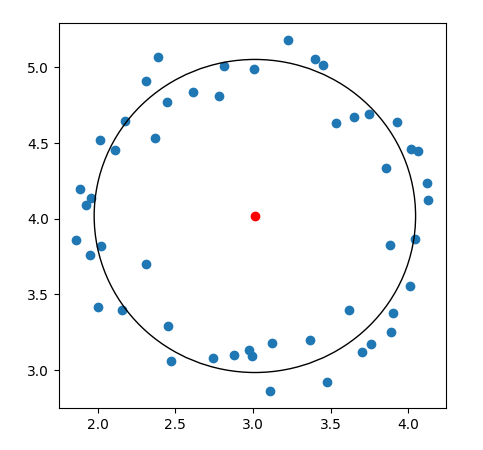
\includegraphics[width=5cm]{circle.png} }}%
    \qquad
    \subfloat[\centering\label{f:end_pose} ]{{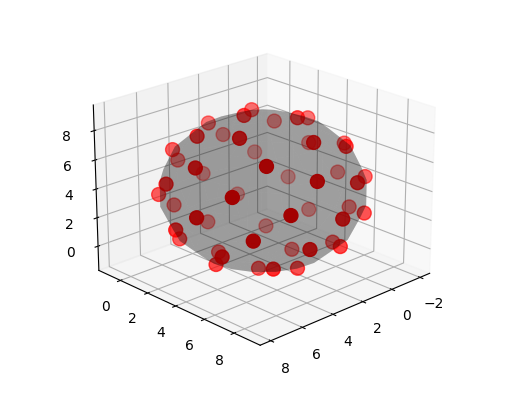
\includegraphics[width=7cm]{shpere.png} }}%
    \label{fig:example}\caption{Expected output for $\mathbb{R}^2$ and $\mathbb{R}^3$} %
\end{figure}

\subsection{Task 05}
Let's try to find the Chebyshev center of a polyhedron. Consider the following polyhedron:
\begin{equation}
    P = \{ x\mid a_i^{\top}x \leq b_i, \; i=1,...,m\}
\end{equation} The Chebyshev center is the center of the largest ball that can fit within the P
\begin{equation}
    Cb = \{ x_c+u\mid \left \| u \right \|_2 \leq r\}
\end{equation}, where $x_c$ is the center and $u = x-x_c$. Hint: Cauchy-Schwarz Inequality: all vectors $\mathbf{a}$ and $\mathbf{u}$ of an inner product space it is true that
\begin{equation}
    \mathbf{a}^T\mathbf{u} \leq \left \| \mathbf{a} \right \|_2 \left \| \mathbf{u} \right \|_2
\end{equation}

\begin{enumerate}
    \item To Cb be inside P, $a_i^{\top}x\leq b_i$ for all $x \subset Cb$, how can you define this condition?
    \item Solve this optimization problem considering these constraints: $A = \begin{bmatrix}
-1 & -1\\ 
-0.5 & 1\\ 
 2& -1
\end{bmatrix}, \; b = \begin{bmatrix}
1\\ 
2\\ 
4
\end{bmatrix}$, and compare your result with MPT toolbox as follows:
    \begin{minted}
[frame=lines, framesep=2mm, baselinestretch=1.2,]
{matlab}

P = Polyhedron('A', A, 'b', b);
hold on
plot(P);
x = sdpvar(2,1);
data = P.chebyCenter(); 
S = YSet(x, norm(x - data.x) <= data.r);
S.plot('color', 'lightgreen');
plot(data.x(1), data.x(2), 'ko', 'MarkerSize'
                    , 10, 'MarkerFaceColor', 'k');
\end{minted} 

\begin{figure}[H]
    \begin{center}
    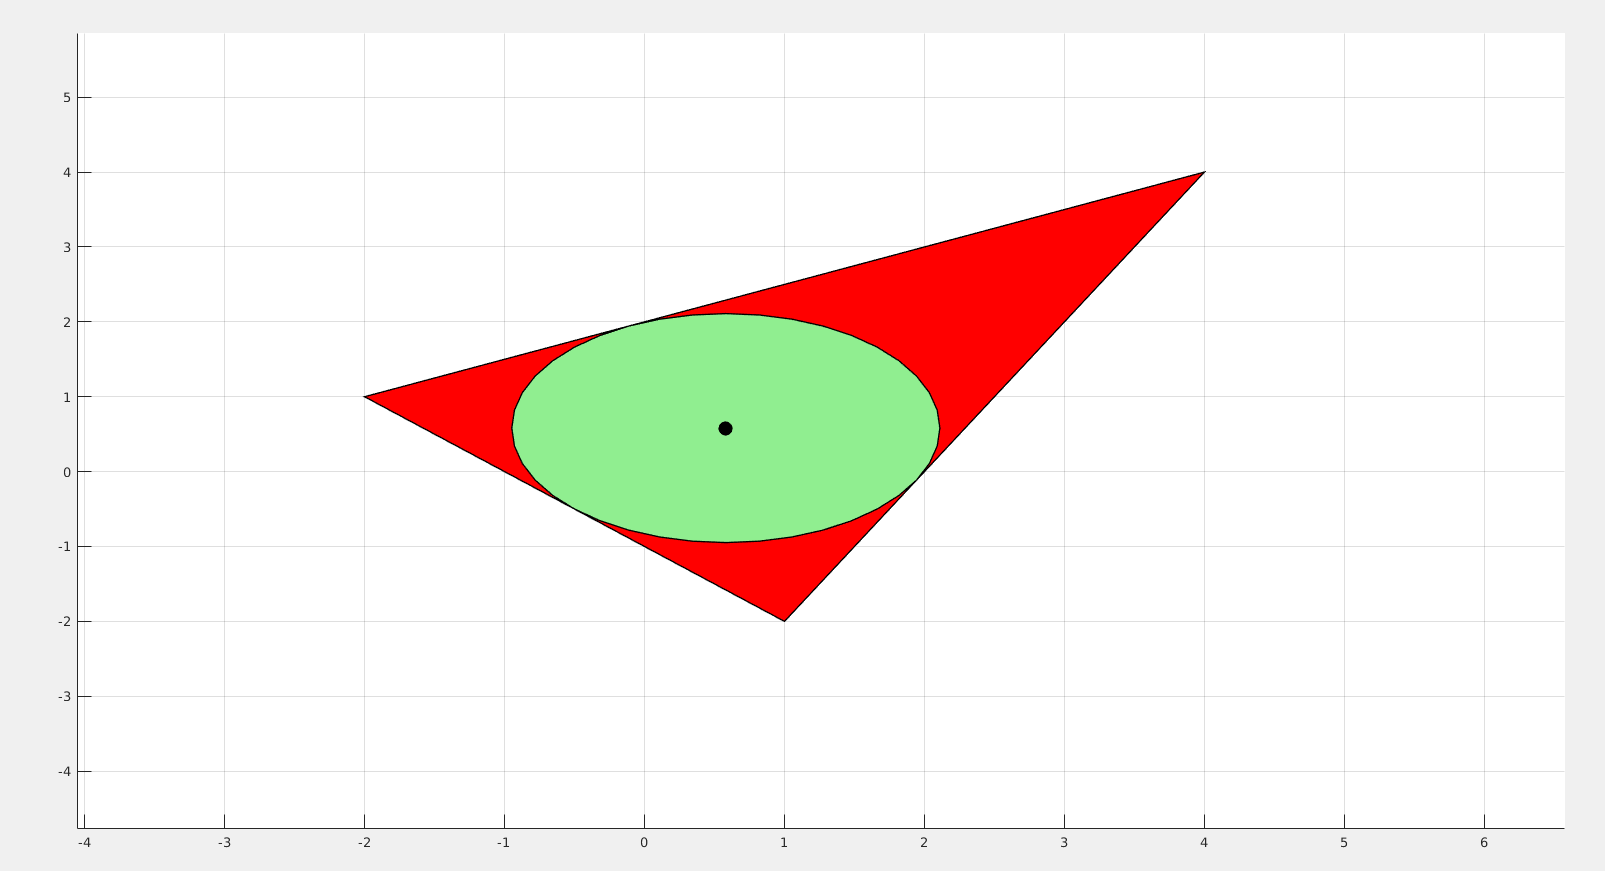
\includegraphics[width=12cm]{ball.png}
    \caption{Chebyshev center}\label{f:farthest-dis}
    \end{center}
\end{figure}
    
\end{enumerate}

\subsection{Task 06}
Let $S=\{y_1\mathbf{a}_1+y_2\mathbf{a}_2 \mid -1<y_1<1, -1<y_2<1\}$, where $\mathbf{a}_1, \mathbf{a}_2 \in \mathbb{R}^n$ be a polyhedron. Your task is to formulate S in the standard form, namely $S=\{ x \mid Ax \leq b, Fx=g\}$. For simplicity assume that $\mathbf{a}_1$ and $\mathbf{a}_2$ are independent, and S can be seen as a intersection of following three sets:
\begin{enumerate}
    \item $S_1$ plane defined by $\mathbf{a}_1$ and $\mathbf{a}_2$
    \item $S_2 = \{ z+y_1\mathbf{a}_1+y_2\mathbf{a}_2 \mid \mathbf{a}_1^Tz=\mathbf{a}_2^Tz=0, \; -1 \leq y_1 \leq 1\}$ parallel to $\mathbf{a}_2$ and orthogonal to $S_1$ 
    \item $S_3 = \{ z+y_1\mathbf{a}_1+y_2\mathbf{a}_2 \mid \mathbf{a}_1^Tz=\mathbf{a}_2^Tz=0, \; -1 \leq y_2 \leq 1\}$ parallel to $\mathbf{a}_1$ and orthogonal to $S_1$ 
\end{enumerate} \textbf{Hint}: a vector $c_1$ that is in the plane that defined by $\mathbf{a}_1$ and $\mathbf{a}_2$, and orthogonal to $\mathbf{a}_2$ can be described by $ c_1 = \mathbf{a}_1 - \frac{\mathbf{a}_1^T\mathbf{a}_2}{\left \| \mathbf{a}_2 \right \|_2^2}\mathbf{a}_2$ 

For visualization you may use following script:
\begin{minted}
[frame=lines, framesep=2mm, baselinestretch=1.2,]
{matlab}
S = Polyhedron('A', A, 'b', b);
plot(S)
\end{minted} 
\begin{figure}[H]
    \begin{center}
    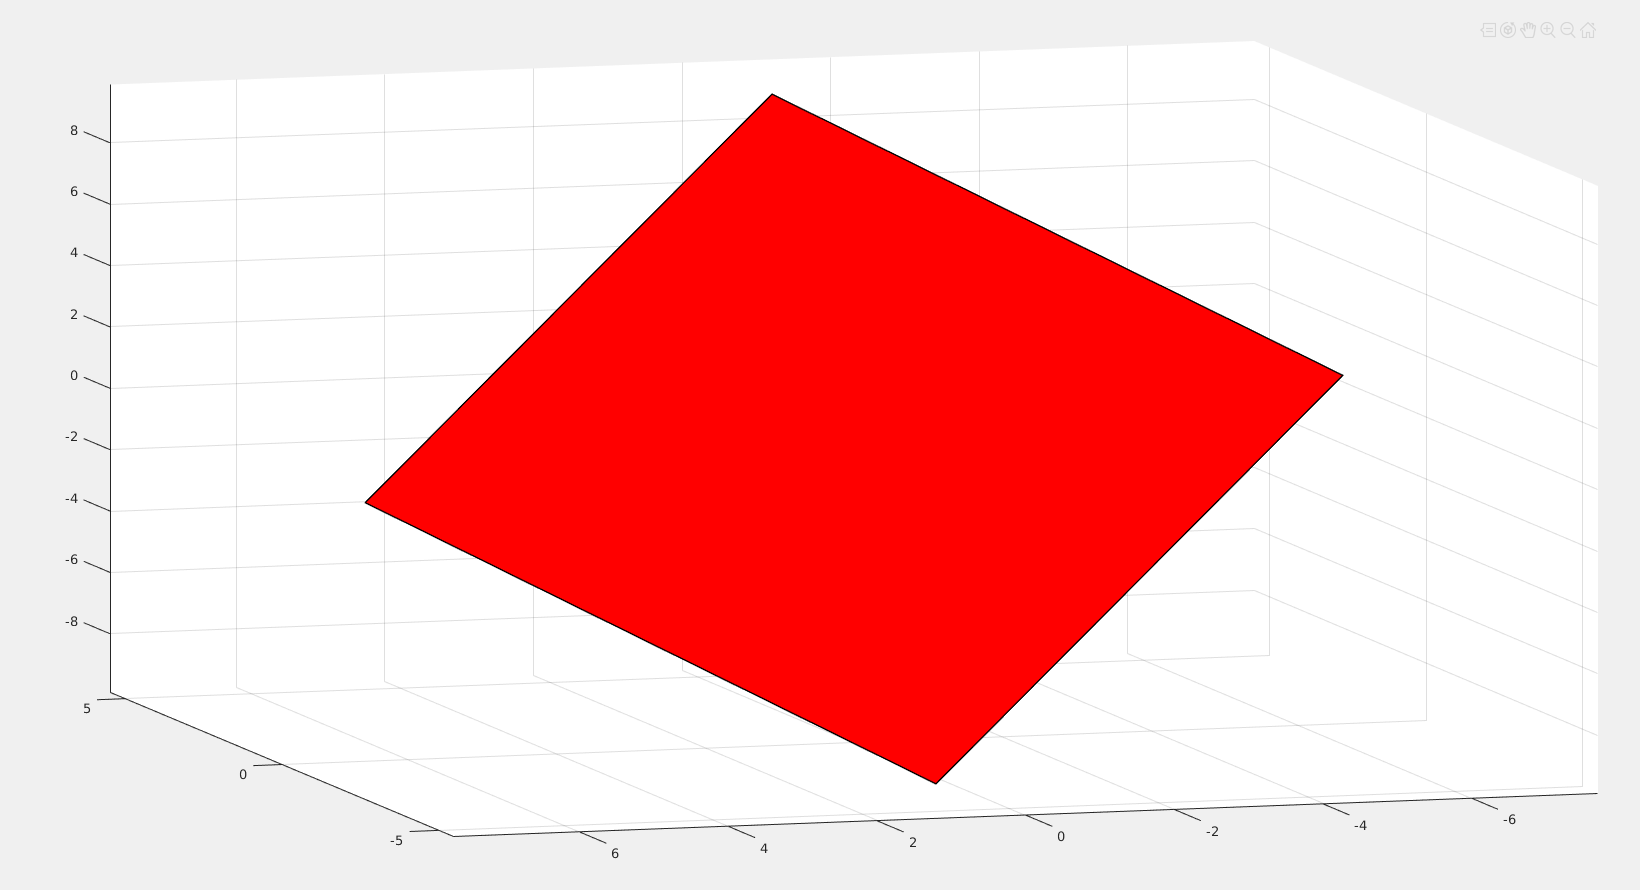
\includegraphics[width=6cm]{polycons.png}
    \caption{S}\label{f:farthest-dis}
    \end{center}
\end{figure}

\section{Appendix A}

\begin{figure}[H]%
    \centering
    \subfloat[\centering \label{f:init_space}  ]{{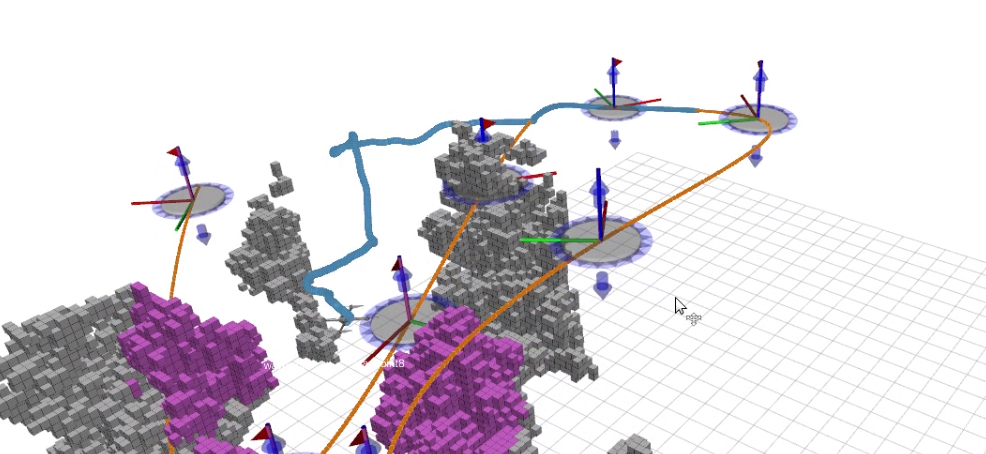
\includegraphics[width=7.5cm]{init_pose.png} }}%
    \qquad
    \subfloat[\centering\label{f:end_pose} ]{{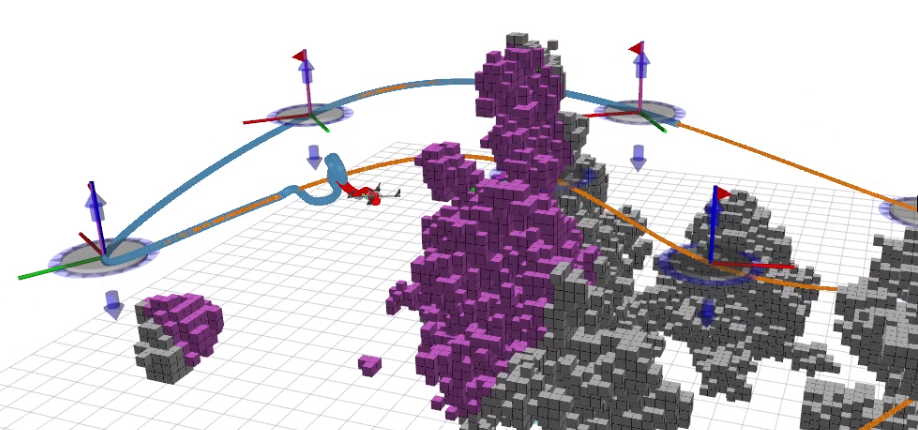
\includegraphics[width=8cm]{end_pose.png} }}%
    \subfloat[\centering\label{f:convex_opt} ]{{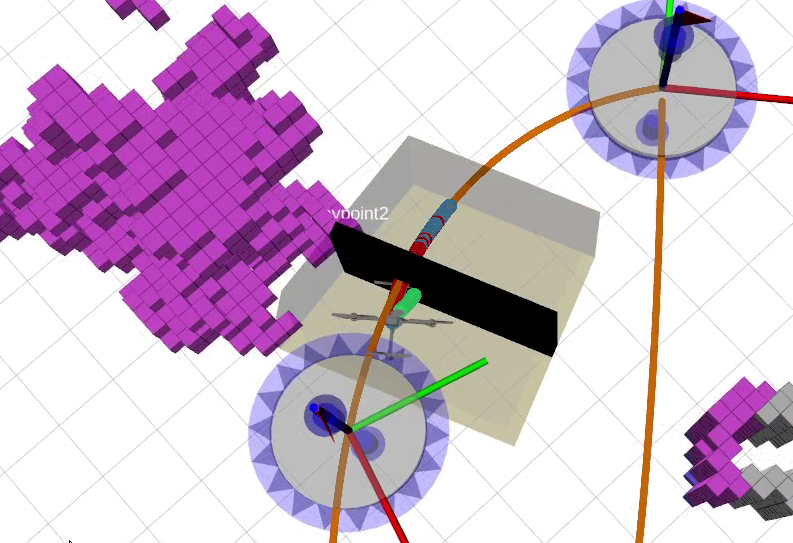
\includegraphics[width=8cm]{convex_opt.png} }}%
    \label{fig:example}\caption{How can we formulate the this trajectory planning as a optimization problem?} %
\end{figure}

\begin{equation}
     J(\Gamma) =  \xi_{obs}J_{obs}(\Gamma) + \xi_{smooth}J_{smooth}(\Gamma) + \xi_{soft}J_{soft}(\Gamma), \quad J_{soft}(\Gamma) = J_{v}(\Gamma) + J_{a}(\Gamma),
\end{equation} where $J_{soft}(\Gamma)$ is determined by soft limits on acceleration and velocity. $J_{smooth}(\Gamma)$ is defined by considering geometric information and/or minimizing snap and/or jerk. $\xi_{obs}J_{obs}(\Gamma)$ helps to avoid collision detection. So how can we define those sub objective functions? What kind of things to be consider? There are so much to think aren't they? Let's get to the problem formulation

\subsection{Convex Set and Convex Functions}
A set $\Omega \subseteq \mathbb{R}^n$ is convex if and only if the line segment between any two points in $\Omega$ lies in $\Omega$, i.e., $\forall x_1,x_2 \Omega$ and $0 \leq \lambda \leq 1$
\begin{equation}
    \lambda x_1 + (1-\lambda)x_2 \in \Omega
\end{equation}$ \lambda x_1 + (1-\lambda)x_2, \; \lambda \in [0,1]$ is called convex combination of $x_1$ and $x_2$. This can be generalized up to n points $\lambda_1 x_1 + ... + \lambda_n x_n, \; \lambda_1 + ...+ \lambda_n = 1$
\begin{figure}[H]
    \begin{center}
    
\includegraphics[width=12cm]{convex_set_non.png}
    \caption{Some convex and nonconvex sets~\cite{boyd2004convex}}
    \end{center}
\end{figure}

A function $f:\mathbb{R}^n \rightarrow \mathbb{R}$ is a convex function if whose domain dom(f) is a convex set and $\forall x,y \in dom(f)$ and $0 \leq \lambda \leq 1$
\begin{equation}
    f(\lambda x_1 + (1-\lambda)x_2) \leq \lambda f(x_1) + (1-\lambda)f(x_2)
\end{equation} Geometrically, the line segments connecting $(x_1, f(x_1))$ to $(x_2, f(x_2))$ is sit above the graph, namely $epi f(x)$ of the function f, refer to Fig.~\ref{f:convex_fun}. Now we are ready to define given optimization problem as convex optimization problem as follows:
\begin{equation}
\begin{aligned}
\min_{} \quad & f(x)\\
\textrm{s.t.} \quad & x \in \Omega,\\
\end{aligned}
\end{equation} where f is a convex function and $\Omega$ is a convex set. Such a problem guarantee to have a global solution due to the convexity nature. 

\begin{figure}[H]
    \begin{center}
    
\includegraphics[width=12cm]{convex-fun.png}
    \caption{Definition of a convex function}\label{f:convex_fun}
    \end{center}
\end{figure}



\subsection{Some importance examples of convex sets}
\subsubsection{Hyperplanes and halfspaces}
Hyperplanes and halfspaces are extremely importance when defining the constrained set for optimization problems. A hyperplane is form as:
\begin{equation}
    Hyperplanes: \{ x|\; a^Tx =b\} \; (a\in \mathbb{R}^n, b \in \mathbb{R}, a\neq 0)
\end{equation} Geometrically, the hyperplanes can be interpreted as the set of points constant inner product to a given vector a (or normal vector) whereas b determine the offset from the origin to the hyperplane. For any point in the hyperplane, namely $x_0$, geometrical interpretation can be understood as \begin{equation}
     \{ x|\; a^T(x-x_0) = 0\} = x_0 + a^{\perp}\; (a\in \mathbb{R}^n, a\neq 0), \quad a^Tx_0 = b, 
\end{equation} where $a^{\perp}$ denotes the orthogonal component of a, i.e., $a^{\perp}=\{ v | a^Tv = 0\}$. This interpretation is illustrated in Fig.~\ref{f:hyperplane_1}.

\begin{figure}[H]
    \begin{center}
    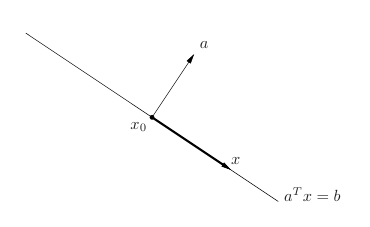
\includegraphics[width=6cm]{hyperplane_1.png}
    \caption{Hyperplane in $\mathbb{R}^2$, with normal vector a and a point $x_0$. THe darker arrow depicts the any point x in the hyperplane, $x-x_0$ ~\cite{boyd2004convex}}\label{f:hyperplane_1}
    \end{center}
\end{figure}


A hyperplanecan be devided into two halfspaces. A closed halfspace is a set of the from
\begin{equation}
    \begin{aligned}
     \{x | a^Tx \leq b\}, \quad a \neq 0, or\\
      \{x | a^T(x-x_0) \leq 0\}, \quad a \neq 0, a^Tx_0 = b\\
     \end{aligned}
\end{equation}. Halfspaces are convex but not affine (Fig.~\ref{f:hyperplane_2})

\begin{figure}[H]
    \begin{center}
    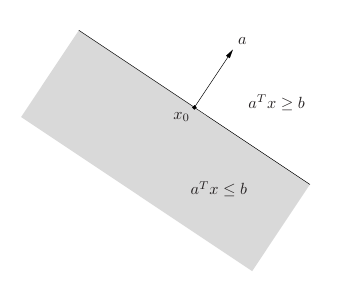
\includegraphics[width=6cm]{hyperplane_2.png}
    \caption{A halfspace determined by $a^Tx \leq b$ ~\cite{boyd2004convex}}\label{f:hyperplane_2}
    \end{center}
\end{figure} The halfspace consists of $x_0$ plus any vector that makes an obtues (or right) angle with the vector a as shown in Fig.~\ref{f:hyperplane_3}.
\begin{figure}[H]
    \begin{center}
    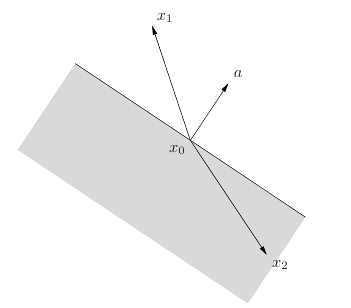
\includegraphics[width=6cm]{hyperplane_3.png}
    \caption{The vector $x_2-x_0$ makes an obtuse angle with a, whereas the vector $x_1-x_0$ makes an acute angle with a. Hence, both $x_1$ and $x_2$ can not be in the halfspace ~\cite{boyd2004convex}}\label{f:hyperplane_3}
    \end{center}
\end{figure}
What is the different between plane and hyperplane? What is the different between hyperplane and halfspace? 



\subsection{Euclidean balls and ellipsoids}
A ball in $\mathbf{R}^n$ has the form
\begin{equation}
    Ball = B(x_c, r) = \{x| \left \| x-x_c \right \|_2 \leq r\} = \{x|(x-x_c)^T(x-x_c) \leq r^2\} = \{x_c+ru| \left \| u \right \|_2 \}\; r>0
\end{equation} Can you try to show ball is a convex set?
A ellipsoid in $x^n \in \mathbf{R}^n$ has the form
\begin{equation}\label{ellipsoid}
    Ellipsoid = \{x | (x-x_c)^TP^{-1}(x-x_c) \leq 1\} = \{x_c+Au|\left \| u \right \|_2 \leq 1 \}\; P=P^T \succ 0
\end{equation} where A is square and nonsingular ($A=P^{1/2}$). The matrix P determines the how far the ellipsoid extends in every direction from $x_c$ whose length is determined by $\sqrt{\lambda_i}$, where $\lambda_i$ is the $i^{th}$ eiegen value. Ellipsoid can be a ball when $P=r^2I$.

\subsection{Polyhedra}
Given the halfspace representation (H-rep), i.e., $Ax \leq b$, corresponding representation is defined in three different ways: Polyhedron ($P = \{x|Ax\leq b\}$), Polyhedral cone ($P={x|Ax\leq 0}$), and Polytope ($P=\{Ax\leq 1\}$). A polyhedron has the form
\begin{equation}
    Polyhedron = \{x|a_jx^T \leq b_j, j=1,...,m, c_j^Tx =d_j, j=1,...,p\} = \{x|Ax \preceq b, Cx=d\}.
\end{equation} Hence, polyhedron is the intersection of a set of halfspaces and hyperplanes. In general, subspaces, hyplerplanes line segments halfspaces are all polyhedra. Let's try to visualize polyhedron, considering following constraints:
\begin{equation}\label{polyconst}
    A = \begin{bmatrix}
 -0.2936  & -1.3260 \\
    0.8245  & -1.4999 \\
    0.1941  &  1.0160 \\
    0.2977  & -0.0275 \\
   -0.7101  & -0.1604 \\
   -0.6877  &  0.3788 \\
    0.5728  & -0.1072 \\
    0.4452  &  0.2128 
\end{bmatrix}, b = \begin{bmatrix}
2.0970 \\
    0.2372 \\
    1.5282 \\
    1.4607 \\
    2.5676 \\
    1.8432 \\
    0.3522 \\
    1.8206 
\end{bmatrix}
\end{equation}

\begin{figure}[H]
    \begin{center}
    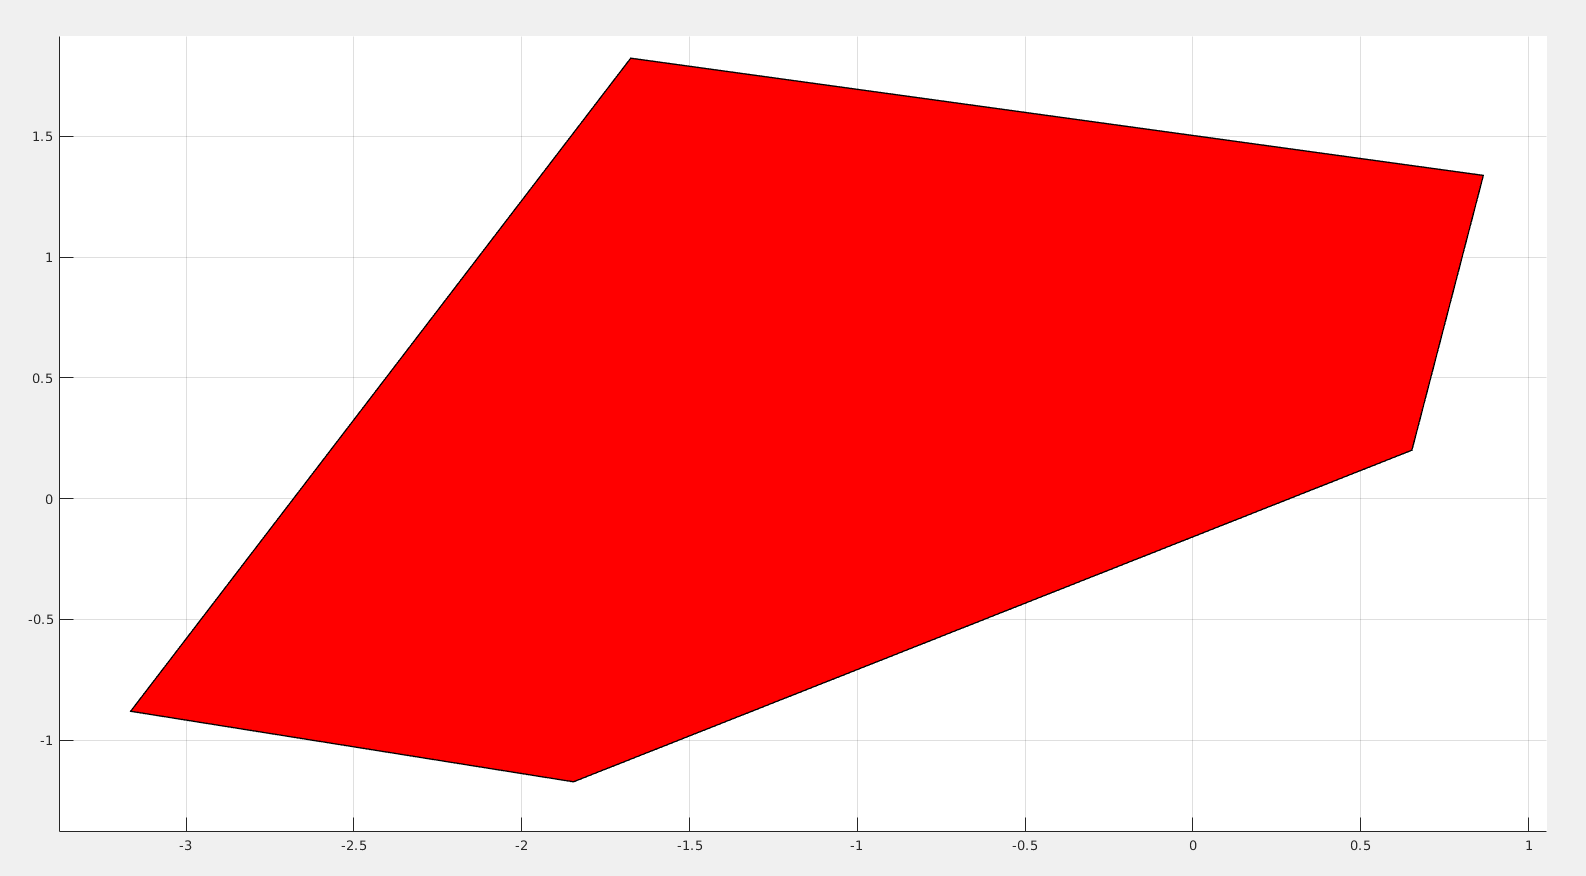
\includegraphics[width=10cm]{polyhedron.png}
    \caption{The polyhedron with respect to (\ref{polyconst})}\label{f:polyhedron}
    \end{center}
\end{figure}

\begin{minted}
[frame=lines, framesep=2mm, baselinestretch=1.2,]
{matlab}
A = randn(8,2);
b = 3*rand(8,1);
P = polytope(A,b);
plot(P);   
\end{minted}    

Let's try to define polyhedron for following constraints set:
\begin{equation}
P = \left\{\begin{matrix}
6x+y \leq 11\\ 
8x+2y \leq 29 \\ 
x-y \geq 11\\ 
2x+y \leq -4\\ 
y \leq 2\\ 
y < 21
\end{matrix}\right.
\end{equation} you may use $P = Polyhedron( 'A', [*], 'b', [*], 'Ae', [*], 'be', *)
$~\cite{poly_ref} notation to define the polyhedron
\subsection{Convex hull of polyhedra}
The convex hull of the given a set of polyhedron is defined as follows:
\begin{equation}
    conv\{v_1,...,v_k\} = \{\theta_1 v_1+...+\theta_k v_k | \theta \succeq 0, 1^T\theta = 1\}
\end{equation}

Let's say you are given a set of points (or vertices) and task is to construct the convex hull with respect to those vertices V and corresponding faces F
\begin{equation}
    V = \begin{bmatrix}
14.2347  & 12.5802 &  13.1171 \\
   12.7639 &  13.2543 &  15.3665 \\
   16.4311  & 15.7984  & 16.0939 \\
   12.1569 &  16.4915 &  16.7446
\end{bmatrix}, \quad F = \begin{bmatrix}
1   &  2  &   4 \\
     1   &  3  &   2 \\ 
     1  &   4  &   3 \\
     2  &   3  &   4 
\end{bmatrix}
\end{equation}

\begin{figure}[H]
    \begin{center}
    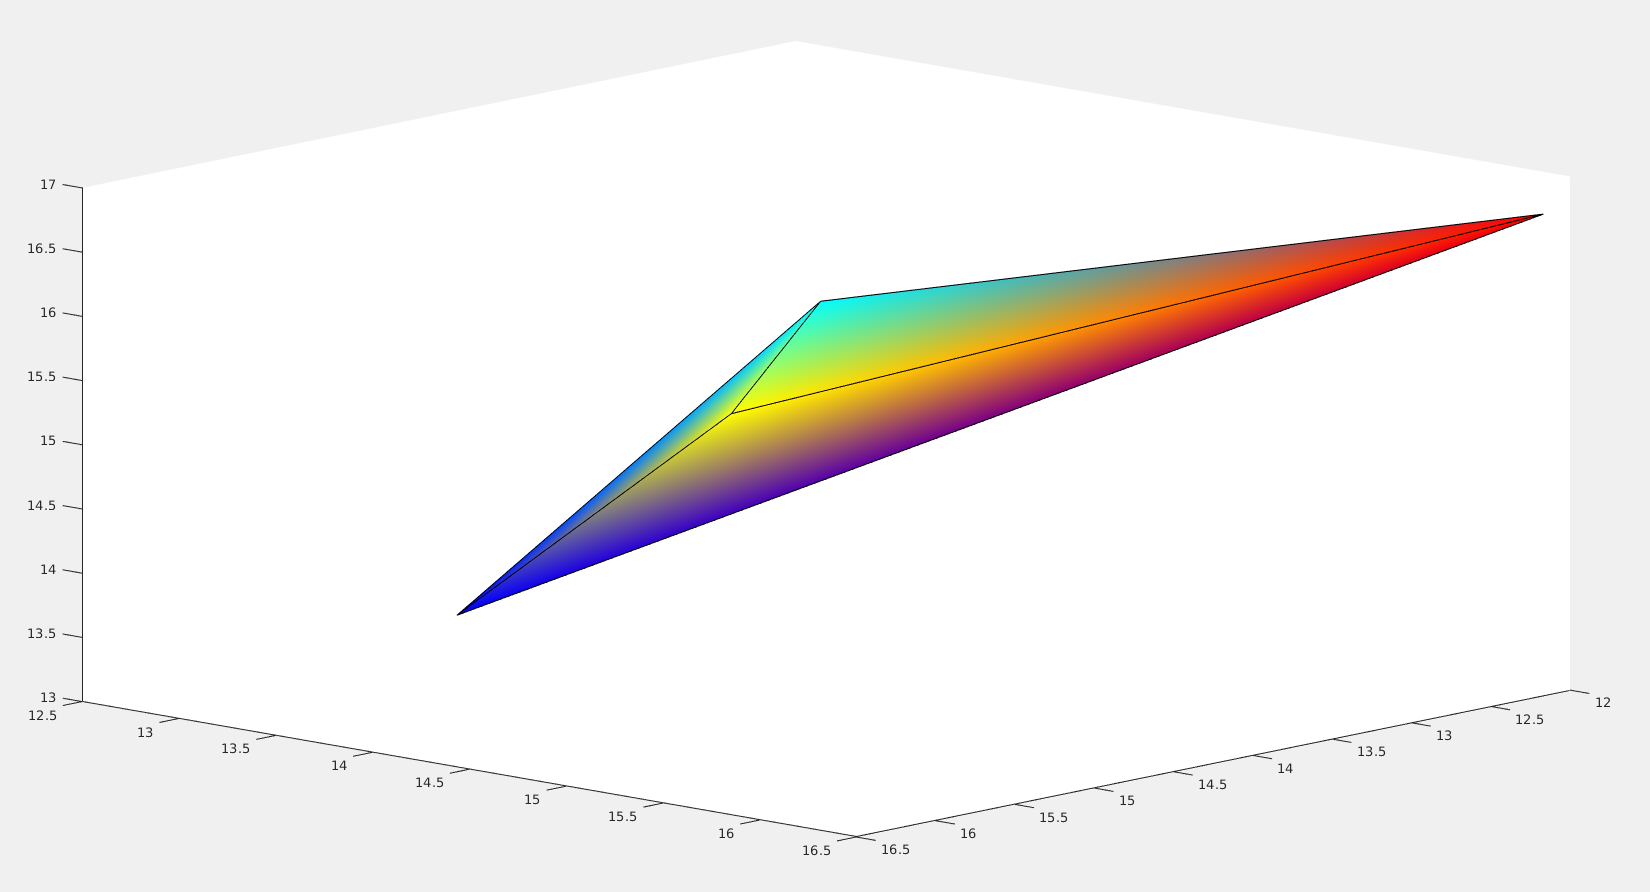
\includegraphics[width=10cm]{convex_hull.png}
    \caption{}\label{f:convex_hull}
    \end{center}
\end{figure}

\begin{minted}
[frame=lines, framesep=2mm, baselinestretch=1.2,]
{matlab}
V = (5).*rand(4,3) + 12;
F = convhull(V);
S.Vertices = V;
S.Faces = F;
S.FaceVertexCData = jet(size(V,1));
S.FaceColor = 'interp';
patch(S); 
\end{minted}  

\subsection{Let's try some operations that preserve convexity}
Minkowski sum or different is interesting property for convex sets. There are various applications in which Minkowski sum is being used. When defining terminal constraints set in  Robust Model Predictive Control (RMPC), Minkowski sum is quite useful. Further, in motion planning, to differentiate free-space from obstacle space this sum is being used. Moreover, in collision detection also this property can be used. 

\begin{minted}
[frame=lines, framesep=2mm, baselinestretch=1.2,]
{matlab}
A = randn(10,2);
b = 3*rand(10,1);
P = polytope(A,b);
hold on
plot(P, 'r');

E = randn(10,2);
f = 0.1*rand(10,1);
S = polytope(E,f);
plot(P-S,'g');
\end{minted} 

\begin{figure}[H]
    \begin{center}
    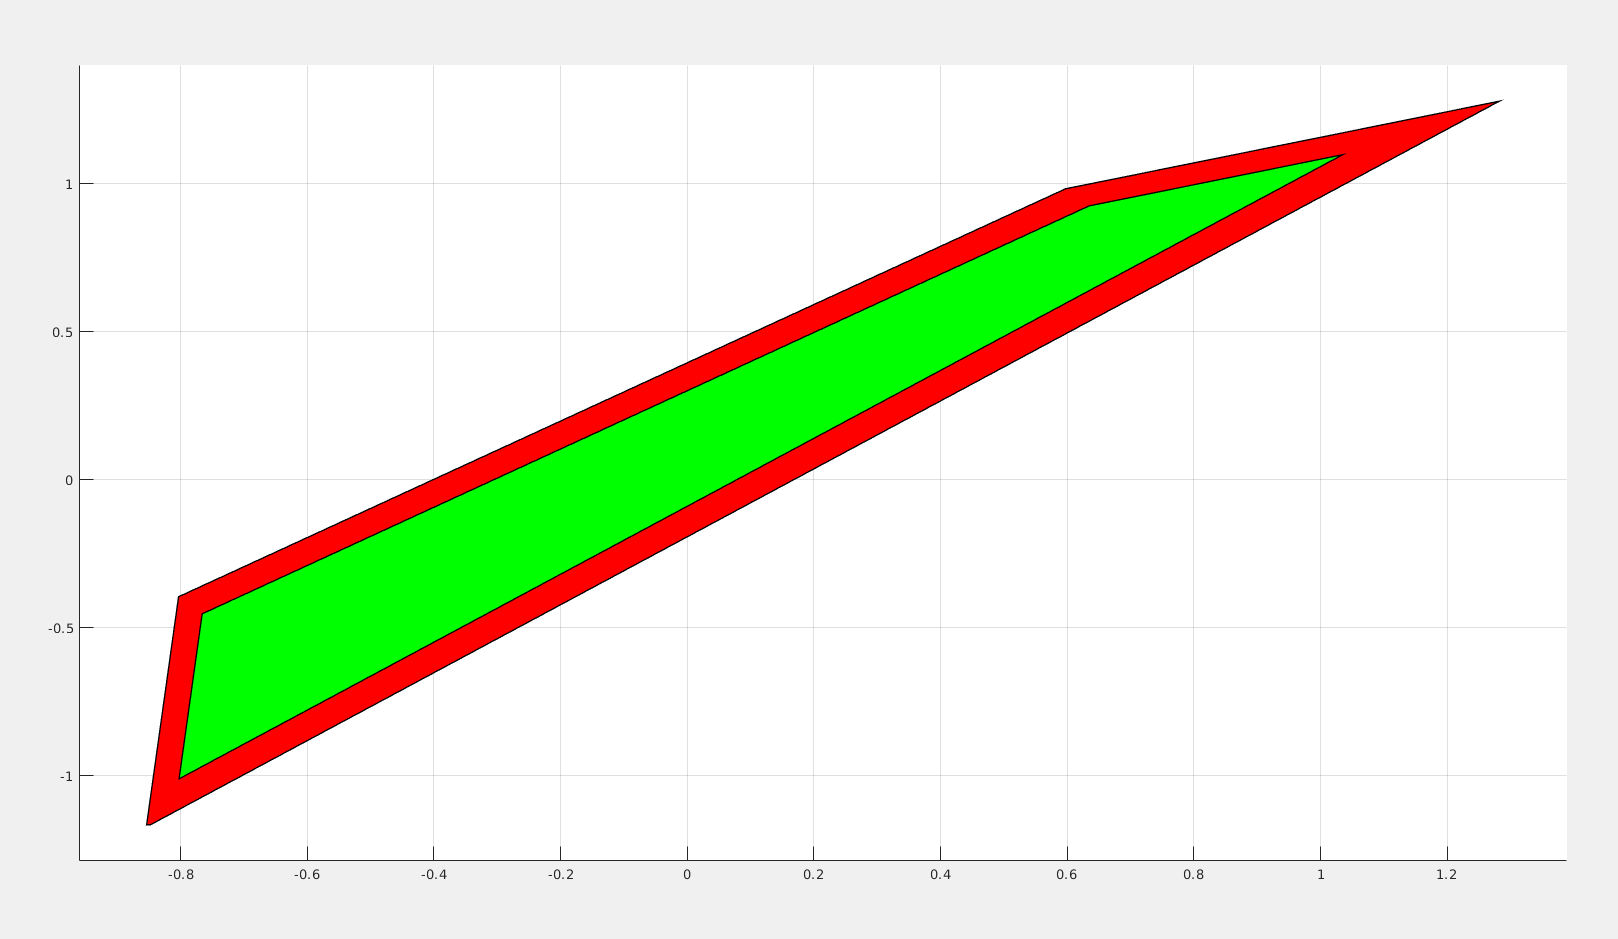
\includegraphics[width=10cm]{minkowski_diff.png}
    \caption{Minkowski difference between two polyhedrons, namely P and E}\label{f:minkowski_diff}
    \end{center}
\end{figure}



Let's try to calculate the center corresponds to inscribing largest ball inside the polyhedron. The ball is described as $\{x | \left \| x-x_c \right \|_2 \leq r\}$. 

\printbibliography
\end{document}